% StrainResponse2q_detail.tex

\tikzstyle{Ellipseobject}=[ultra thick, draw=blue, ellipse, minimum width=24em,
    minimum height=8em,align=center]
\tikzstyle{EllipseStallObject}=[ultra thick, draw=blue, ellipse, minimum width=12em,
    minimum height=8em,align=center]
\tikzstyle{LabelObject}=[draw=black, fill=white,rectangle,rounded corners,line width=0.5mm,%
	  align=center]
\tikzstyle{ArrowObject}=[red,line width=1.0mm, -latex]
\tikzstyle{WingRoot}=[draw=black, fill=white,rectangle,line width=0.25mm,%
	  align=center,minimum width=0.25em,minimum height=4.5em,pattern=north west lines]
\tikzstyle{WingPlanform}=[draw=black, fill=white,rectangle,line width=0.25mm,%
	  align=center,minimum width=14.24em,minimum height=3em]
\tikzstyle{SecObject}=[draw=black, rectangle,line width=0.25mm,%
	  align=center,minimum width=1em,minimum height=3em]
\tikzstyle{SelSecObject}=[draw=black, fill=blue,rectangle,line width=0.25mm,%
	  align=center,minimum width=1em,minimum height=3em]
\tikzstyle{SGObject}=[draw=black, rectangle,line width=0.25mm,%
	  align=center,minimum width=1em,minimum height=1em]
\tikzstyle{SelSGObject}=[draw=black, fill=blue,rectangle,line width=0.25mm,%
	  align=center,minimum width=1em,minimum height=1em]

\resizebox{!}{0.3\textwidth}{
	\begin{tikzpicture}
		\only<1,2>{
			\node[anchor=south west,inner sep=0] (image) at (0,0)%
				{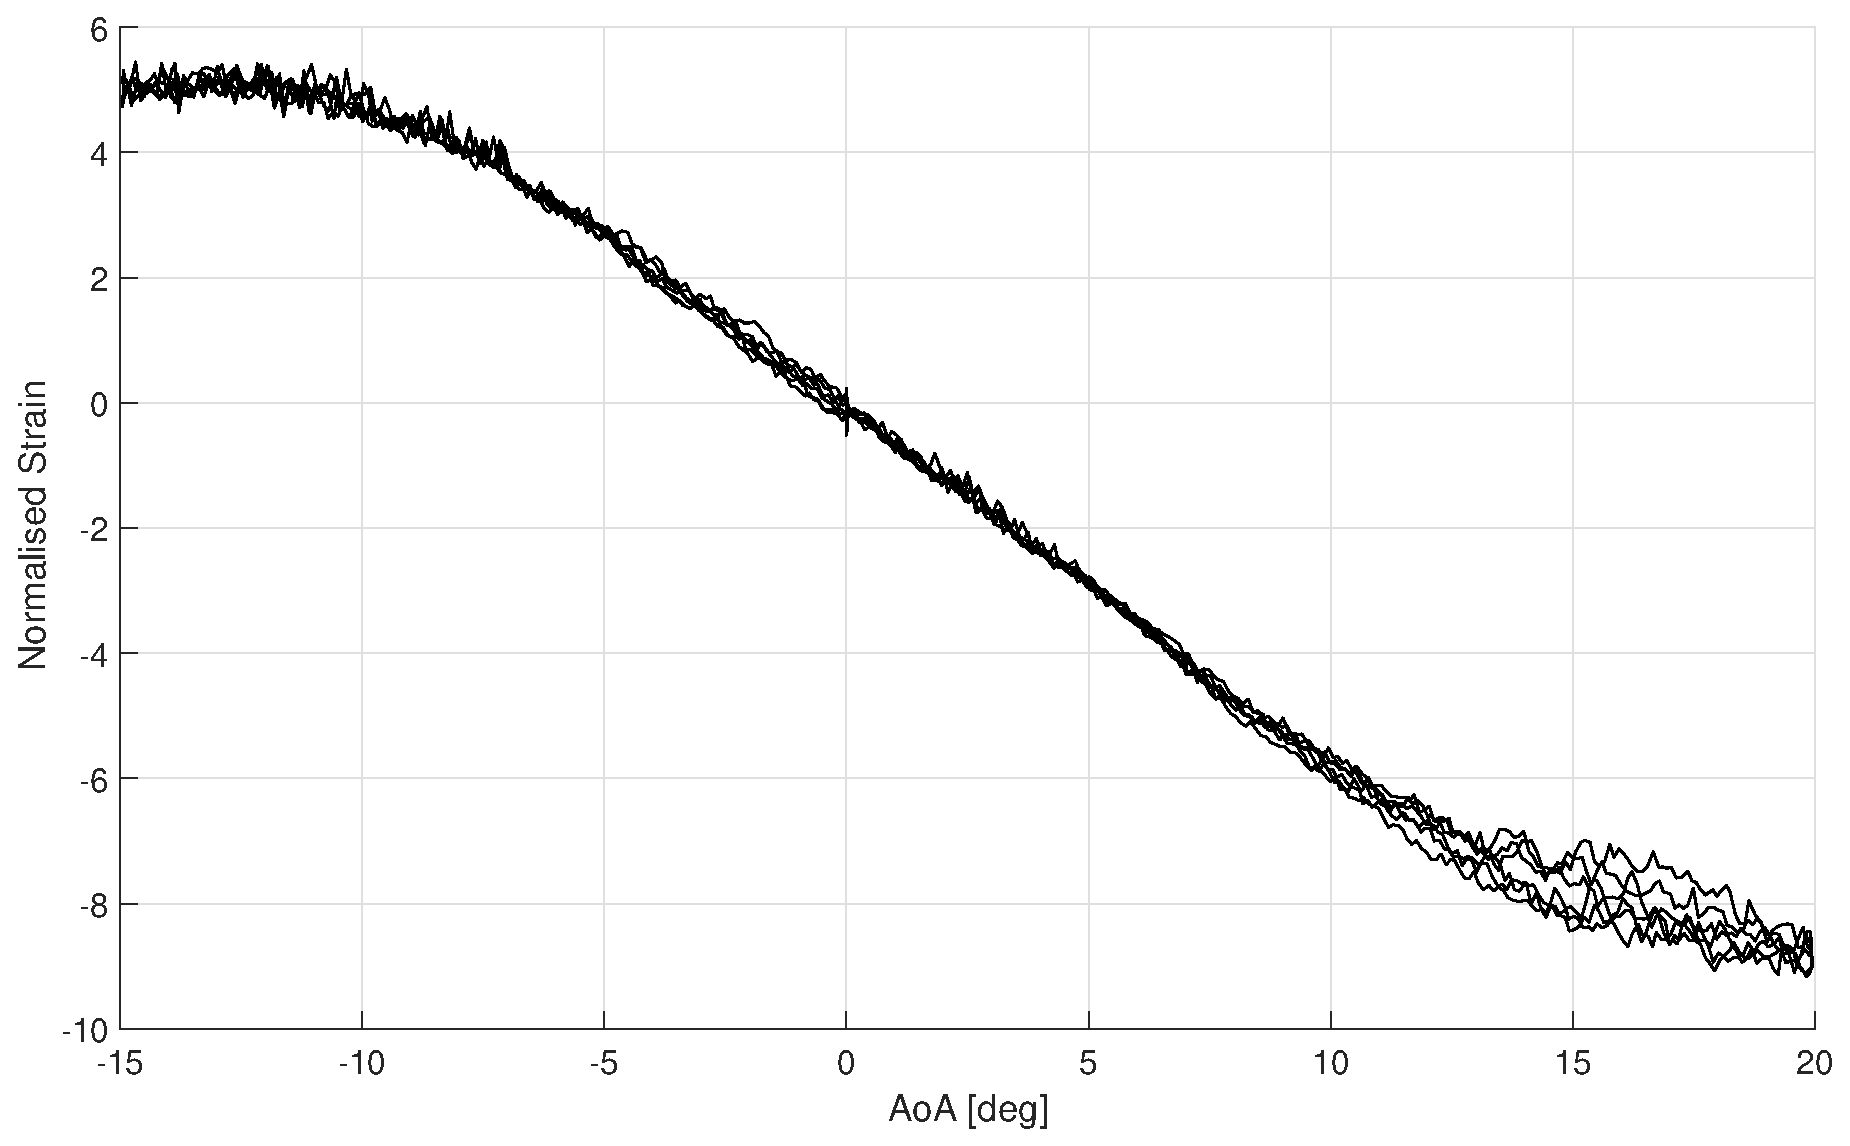
\includegraphics[width=\textwidth]{DistDataSet_P07.eps}};
		}
		\only<3>{
			\node[anchor=south west,inner sep=0] (image) at (0,0)%
				{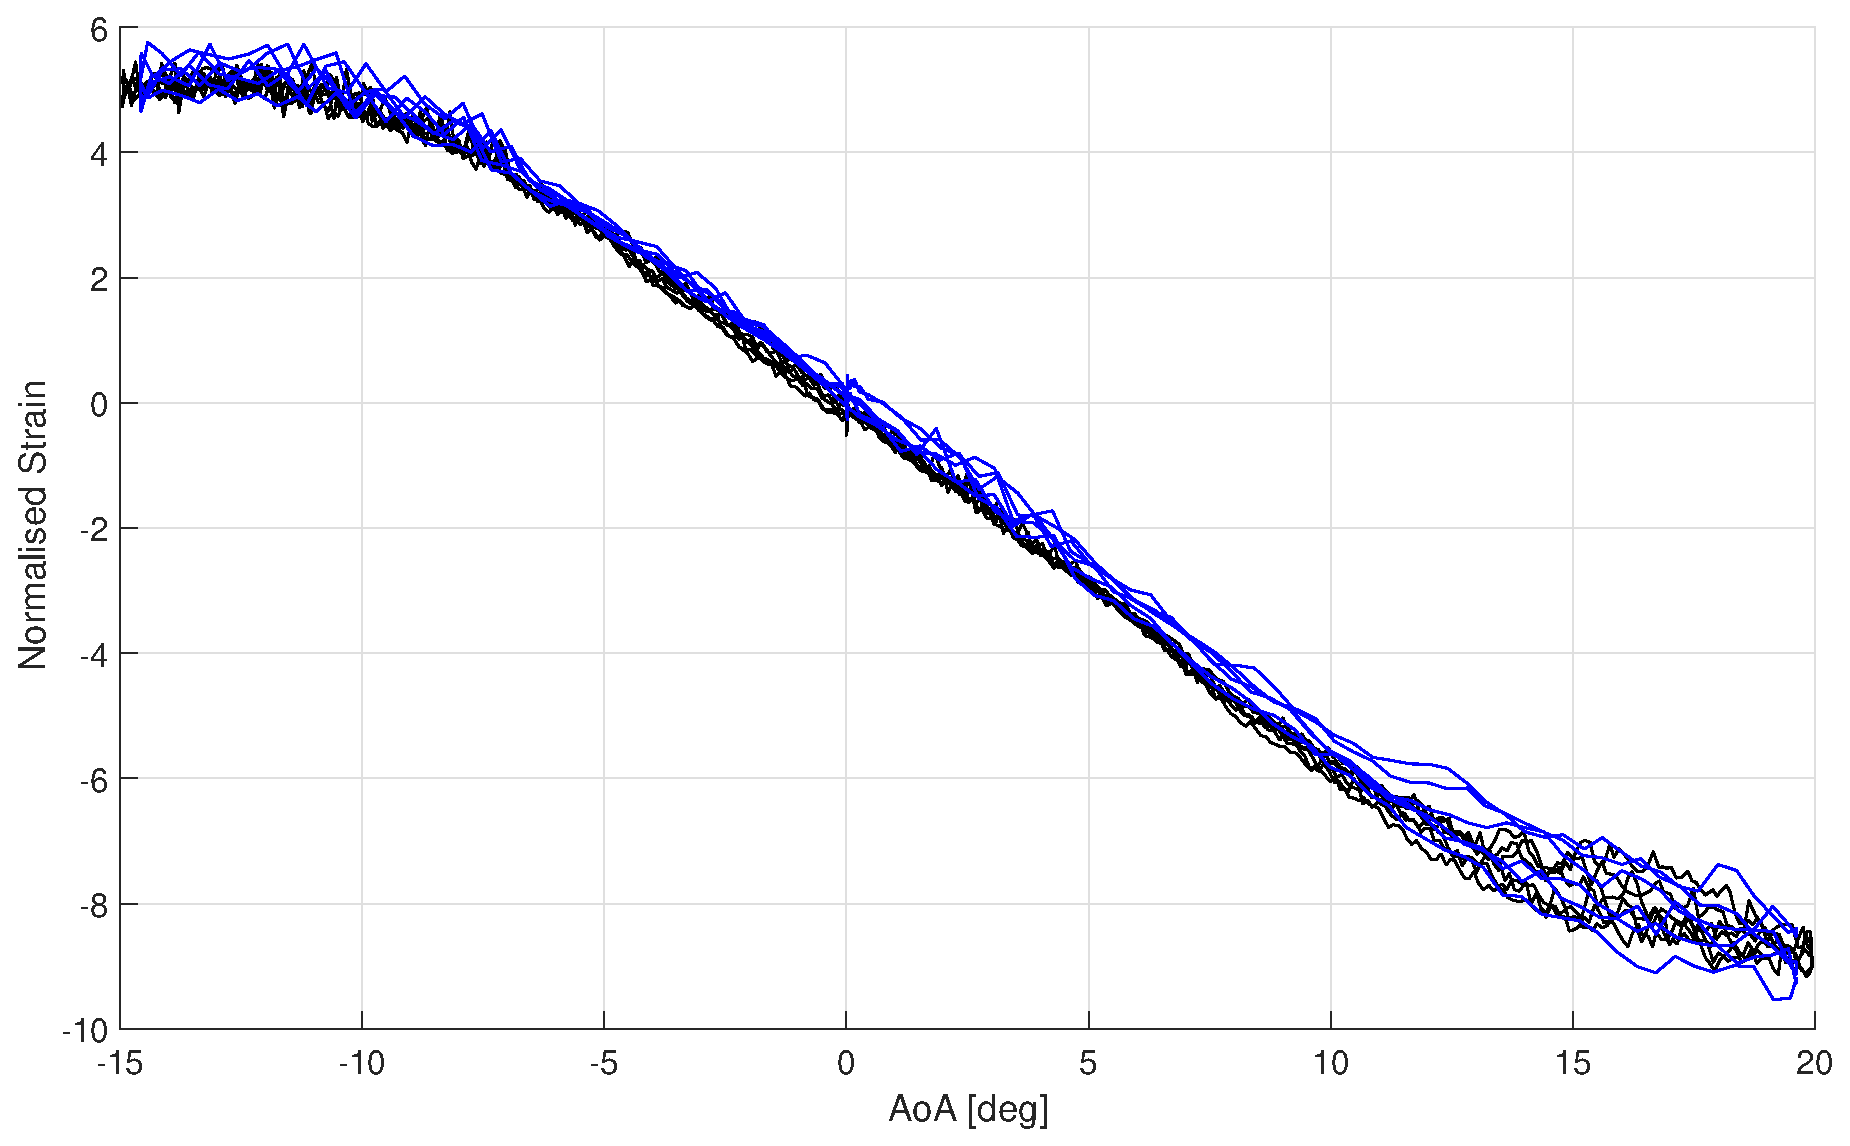
\includegraphics[width=\textwidth]{DistDataSet_P08.eps}};
		}
		\only<4->{
			\node[anchor=south west,inner sep=0] (image) at (0,0)%
				{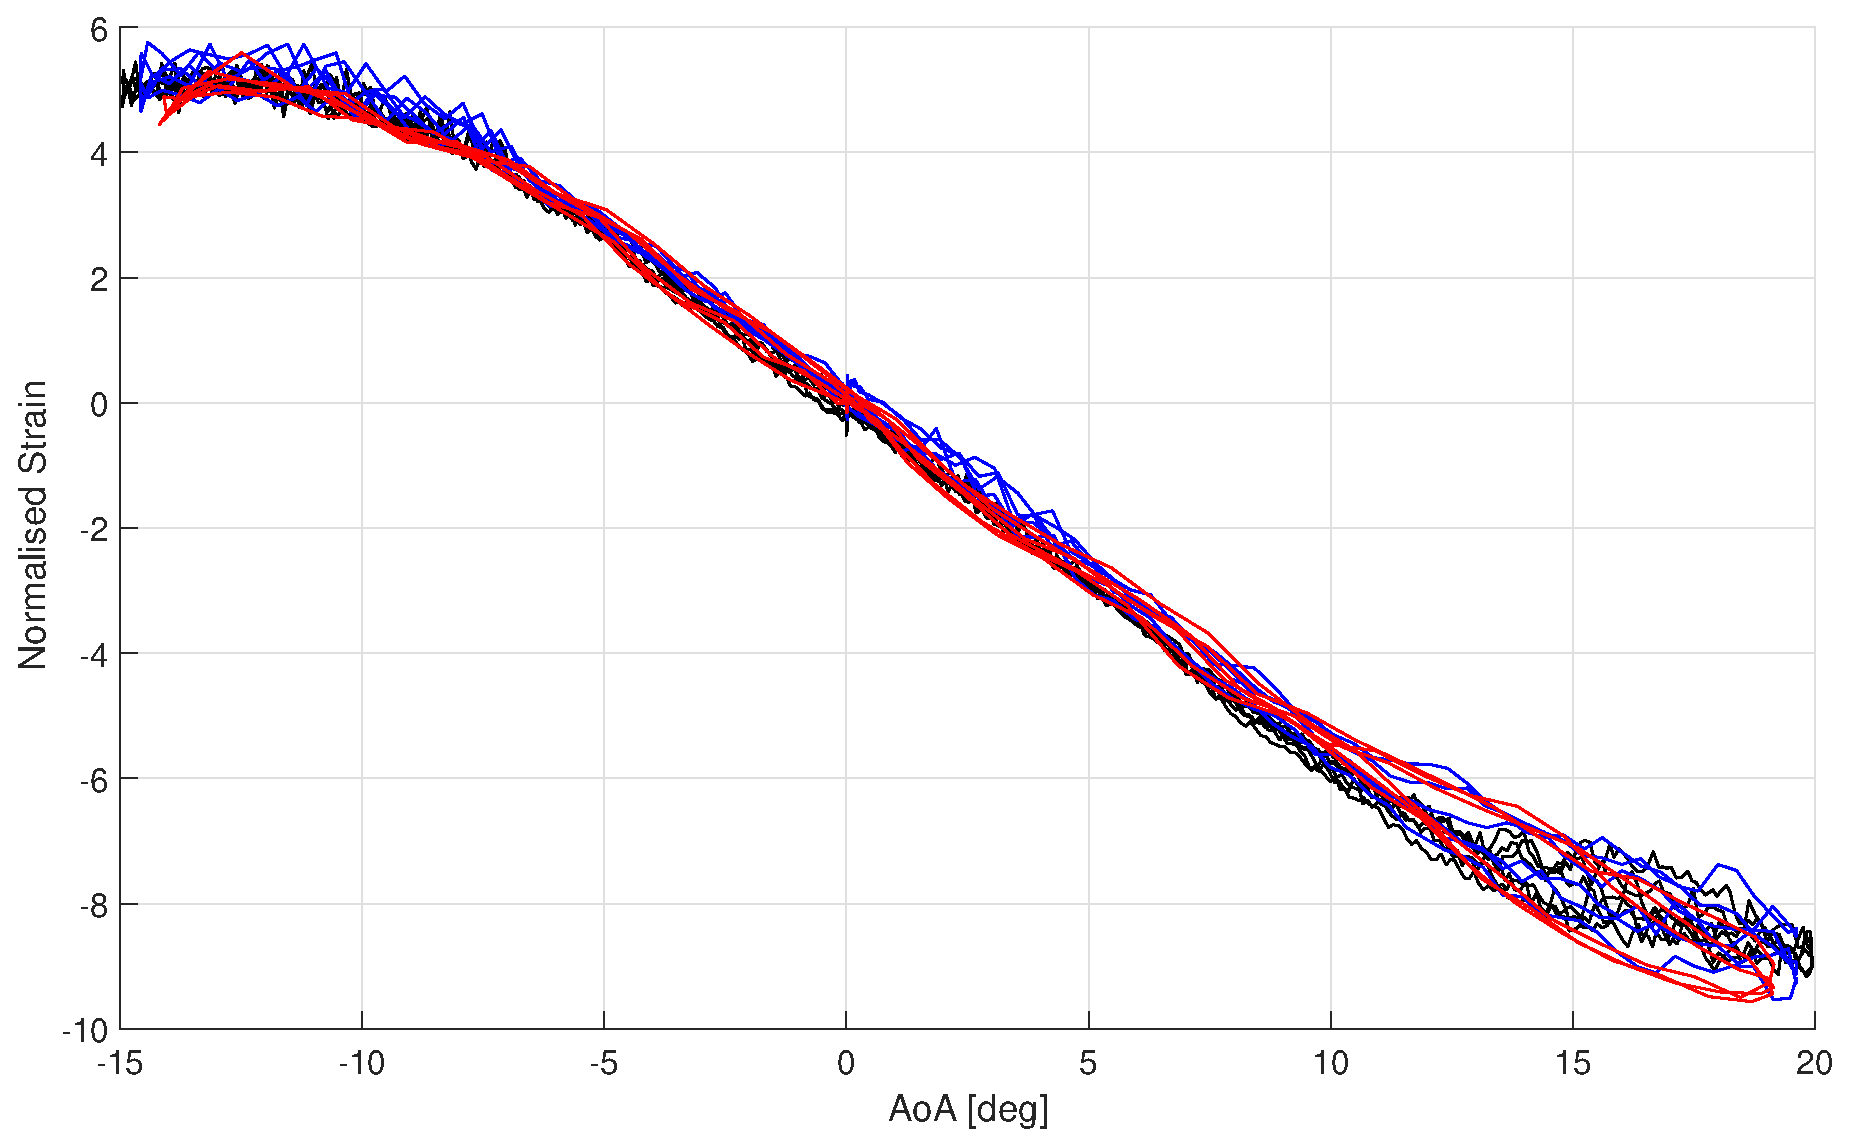
\includegraphics[width=\textwidth]{DistDataSet_P09.eps}};
		}
		\only<5>{
			\node[anchor=south west,inner sep=0] (image) at (0,0)%
				{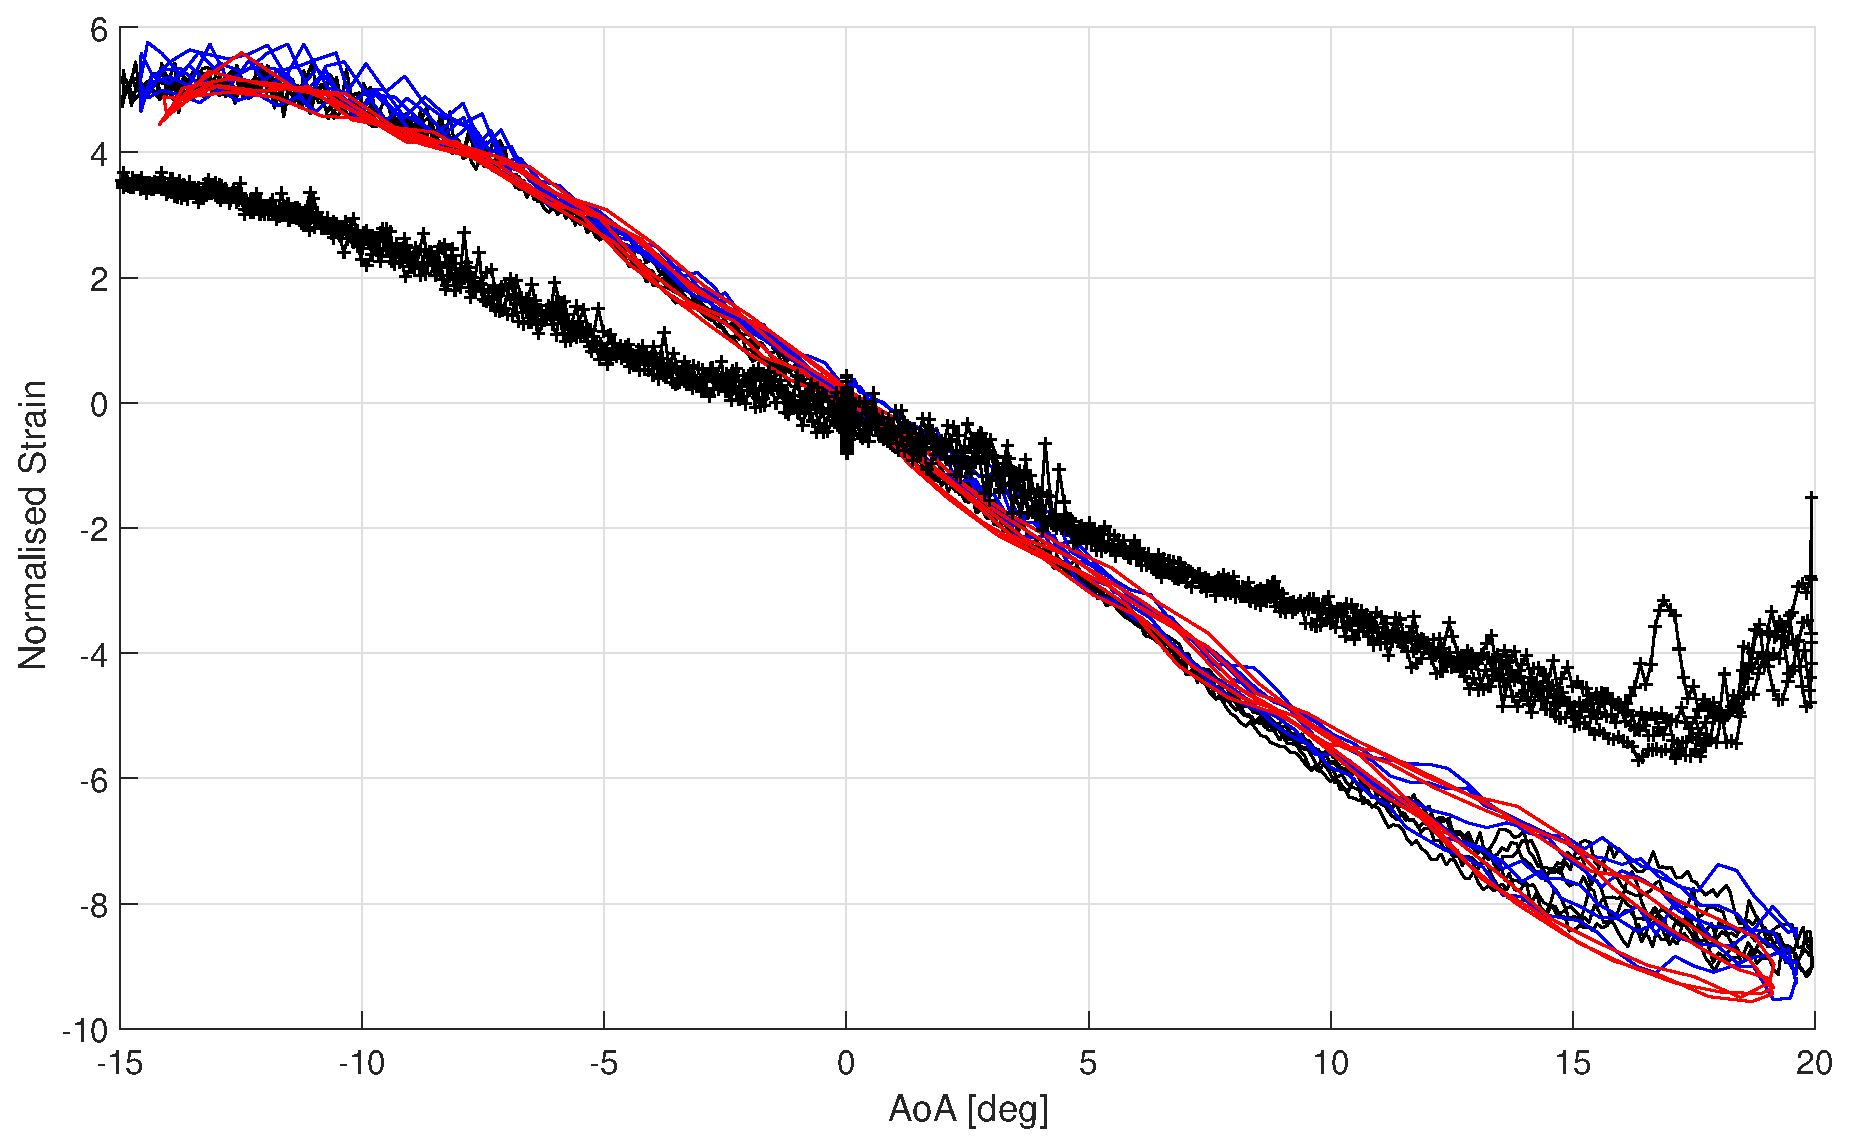
\includegraphics[width=\textwidth]{DistDataSet_P10.eps}};
		}
		\only<6>{
			\node[anchor=south west,inner sep=0] (image) at (0,0)%
				{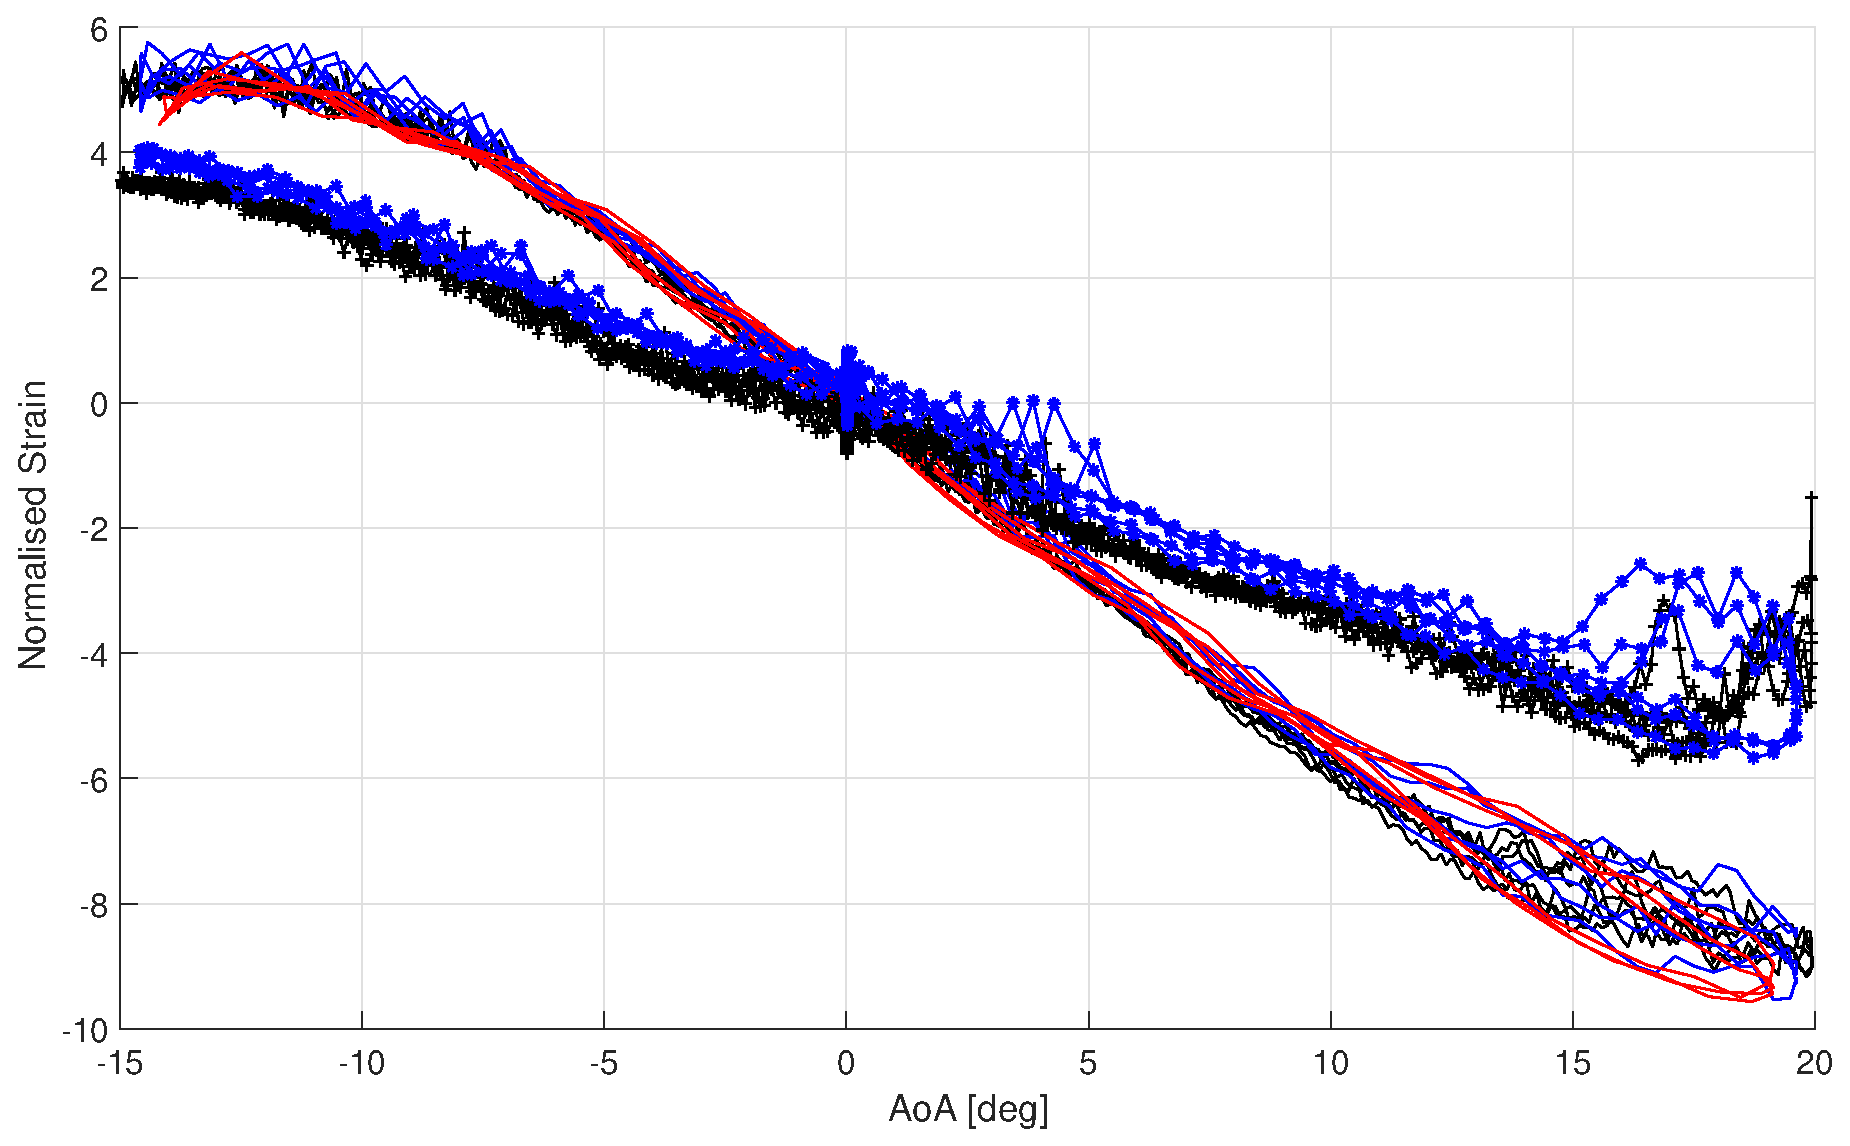
\includegraphics[width=\textwidth]{DistDataSet_P11.eps}};
		}
		\only<7>{
			\node[anchor=south west,inner sep=0] (image) at (0,0)%
				{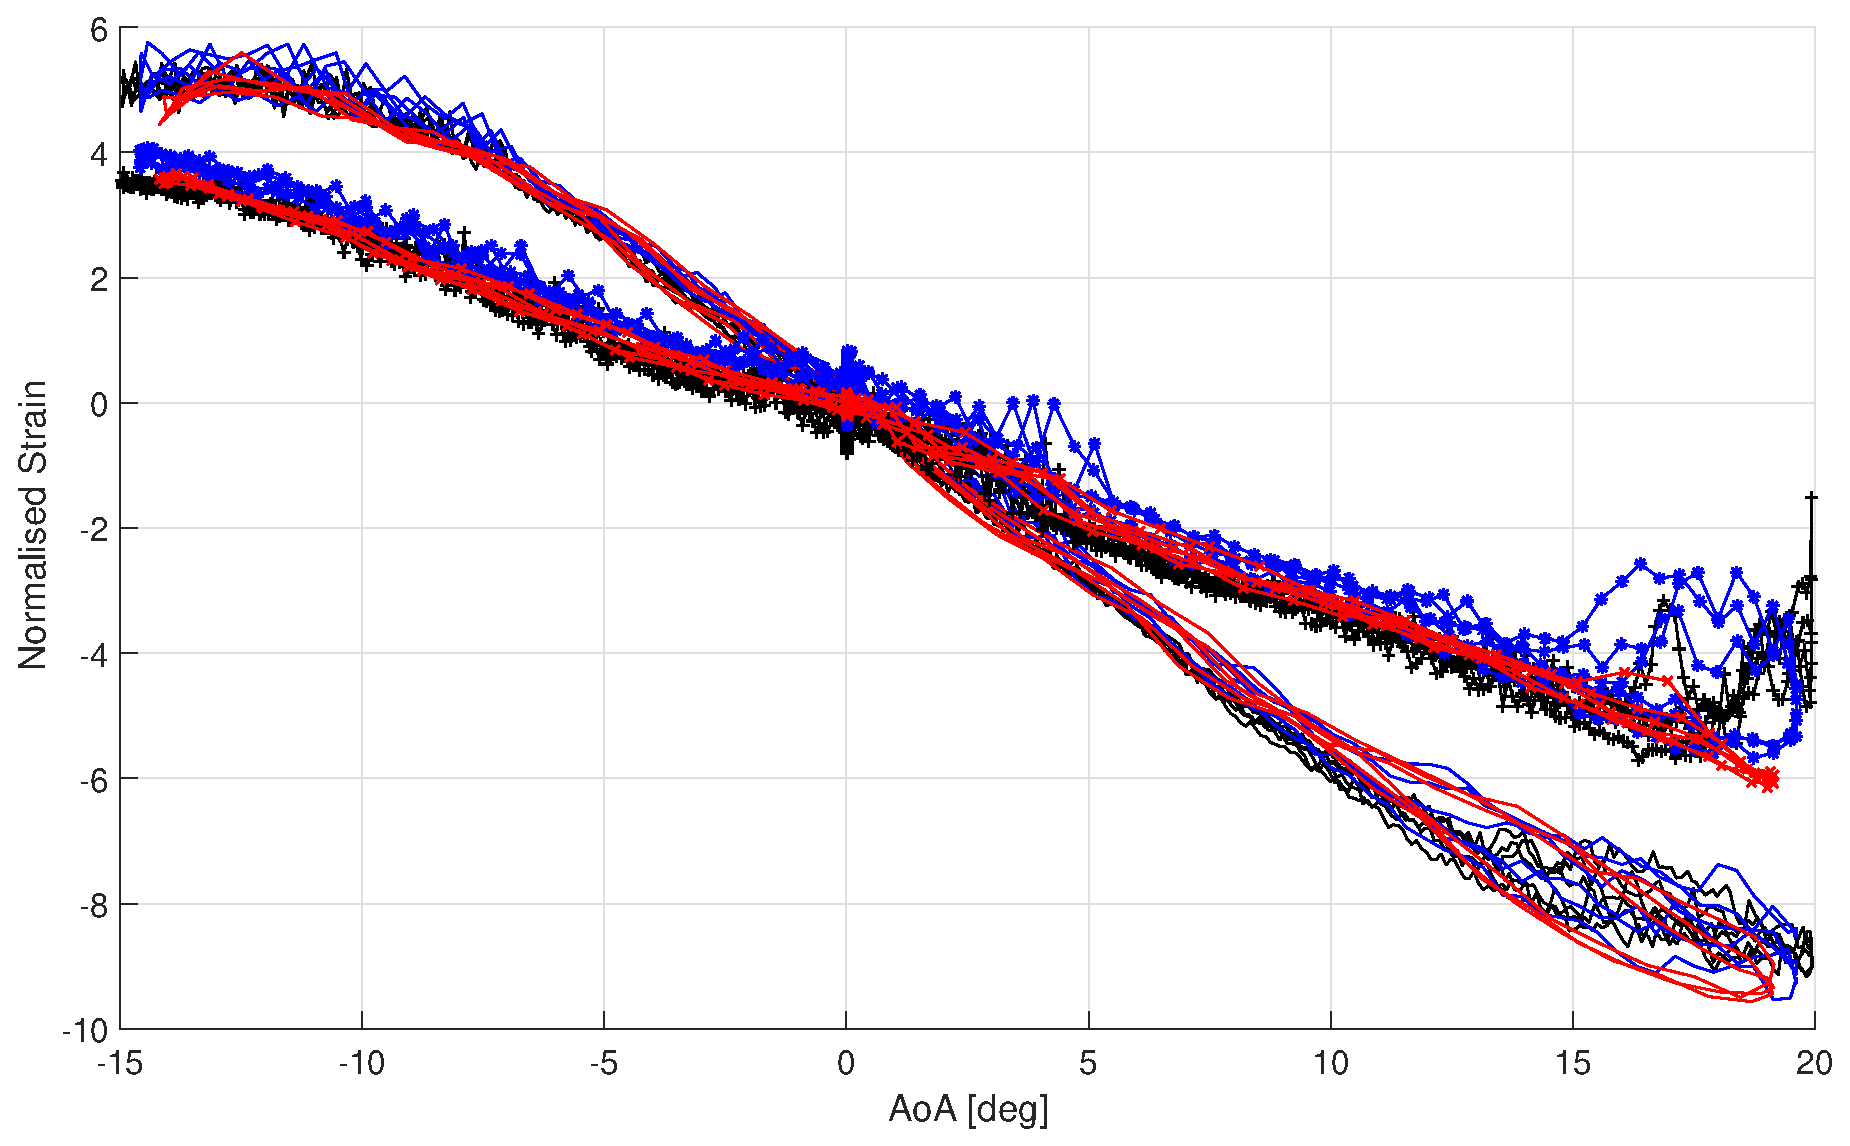
\includegraphics[width=\textwidth]{DistDataSet_P12.eps}};
		}
		% Define scope with 'image' dimensions as reference
		\begin{scope}[x={(image.south east)},y={(image.north west)}]
			%\draw[help lines,xstep=.05,ystep=.05] (0,0) grid (1,1);
			%\foreach \x in {0,1,...,9} { \node [anchor=north] at (\x/10,0) {0.\x}; }
			%\foreach \y in {0,1,...,9} { \node [anchor=east] at (0,\y/10) {0.\y}; }
			
			% Wing node
			\draw(0.8,0.905) node (WingNode) {};
			% Wing instance
			\node[WingPlanform] (WingPlanform) at (WingNode) {};
			\draw (WingNode) ++(-0.165,0) node[WingRoot] (WingRoot) {};
			\draw (WingNode) ++(-0.075,0) node[SecObject] (SecB) {};
			\draw (WingNode) ++(+0.075,0) node[SecObject] (SecA) {};
			\draw (WingNode) ++(-0.115,0) node[SGObject] (SG_A) {};
			\draw (WingNode) ++(-0.045,0) node[SGObject] (SG_B) {};
			\draw (WingNode) ++(+0.045,0) node[SGObject] (SG_C) {};
			\draw (WingNode) ++(+0.115,0) node[SGObject] (SG_D) {};
			\only<1,2,3->{
			  %
				\draw (WingNode) ++(-0.115,0) node[SelSGObject] (SG_A) {};
			}
			%\only<4->{
			  %%
				%\draw (WingNode) ++(+0.045,0) node[SelSGObject] (SG_C) {};
			%}
			% Legend Nodes
			\draw(0.20,0.30) node (q0_Line) {};
			\draw(0.20,0.25) node (q1_Line) {};
			\draw(0.20,0.20) node (q2_Line) {};
			% Legend Arrows & Labels
			\only<1->{
			  \draw[black,line width=0.5mm] (q0_Line) -- +(-0.1,0);
				\draw(q0_Line) ++(+0.080,0) node (q0_Label) {$q = \SI[per-mode=symbol]{\pm 0.5}{\degree\per\second}$};
			}
			\only<3->{
			  \draw[blue, line width=0.5mm] (q1_Line) -- +(-0.1,0);
				\draw(q1_Line) ++(+0.075,0) node (q1_Label) {$q = \SI[per-mode=symbol]{\pm 20}{\degree\per\second}$};
			}
			\only<4->{
			  \draw[red,  line width=0.5mm] (q2_Line) -- +(-0.1,0);
				\draw(q2_Line) ++(+0.075,0) node (q2_Label) {$q = \SI[per-mode=symbol]{\pm 50}{\degree\per\second}$};
			}
			
			\only<2>{
			  % Linear Strain node
			  \draw(0.475,0.625) node (StrainAoA) {};
			  % Linear Strain marker
			  \node[Ellipseobject,rotate around={-35:(0,0)}] (StrainLinAoA) at (StrainAoA) {};
				% Linear Strain label
			  \draw(0.9,0.7) node[LabelObject] (StrainLinAoA_Label) {Strain Linear\\Response\\with AoA};
			  % Linear Strain arrow
			  \draw[ArrowObject] (StrainLinAoA_Label.west) -- (StrainLinAoA.north);
			}
			\only<5>{
			  % Linear Strain node
			  \draw(0.85,0.2) node (DynamicLift_Node) {};
			  % Linear Strain marker
			  \node[EllipseStallObject,rotate around={-25:(0,0)}] (DynamicLift) at (DynamicLift_Node) {};
				% Linear Strain label
			  \draw(0.85,0.7) node[LabelObject] (DynamicLift_Label) {Dynamic Lift};
			  % Linear Strain arrow
			  \draw[ArrowObject] (DynamicLift_Label.south) -- (DynamicLift.north);
			}
		\end{scope}
	\end{tikzpicture}
}